\heading{固体物理学-24秋-期中}
\noteinfo{题面依据原始扫描件精修录入；原件夹有参考作答，但未直接照录；现有解答为依据题面重新推导的参考答案。个别不完整表述已在不改变考查内容的前提下删改。}

\textbf{一、填空题（每空答错扣 1 分，扣完为止）}

\begin{question}
晶体中两种常见密排结构的堆积致密度均为 \blank。


\begin{solution}
最密堆积中每个球有 12 个最近邻。以面心立方惯用胞计算：胞内有 4 个球，面对角线满足 $\sqrt2a=4R$，故
\[
 \eta=\frac{4\times\frac43\pi R^3}{a^3}
 =\frac{\pi}{3\sqrt2}\simeq0.7405.
\]
六方最密堆积具有相同的局域堆积，故
\[
 \boxed{\eta_{\rm FCC}=\eta_{\rm HCP}=\frac{\pi}{3\sqrt2}\approx74\%.}
\]
\end{solution}
\end{question}

\begin{question}
布拉格定律为 \blank；布里渊区边界由满足布拉格反射条件的波矢端点构成。


\begin{solution}
相邻晶面散射波的光程差为 $2d\sin\theta$。相长干涉要求它等于整数倍波长，因此
\[
 \boxed{2d\sin\theta=n\lambda,\qquad n=1,2,\ldots}
\]
这就是 Bragg 定律。等价地，弹性散射满足 Laue 条件
$\vb k'-\vb k=\vb G$；其几何边界正是倒空间中到原点和某倒格点等距的布拉格面。
\end{solution}
\end{question}

\begin{question}
对晶格常数为 $a$ 的简单立方晶体，求与正格矢
\[
  \vb R=a\vb i+2a\vb j+3a\vb k
\]
正交的倒格子晶面族的晶面指数及其晶面间距。


\begin{solution}
本题所说“倒格子晶面与正格矢 $\vb R$ 正交”，应理解为倒空间晶面法向平行于该正格矢。简单立方正、倒格基矢分别满足
\[
 \vb a_i=a\hat{\vb e}_i,
 \qquad \vb b_i=\frac{2\pi}{a}\hat{\vb e}_i.
\]
给定
$\vb R=a(1,2,3)$，故与之垂直的倒格子晶面族的法向指标为
\[
 \boxed{(123)_{\rm reciprocal}.}
\]
在倒空间中，相邻该晶面间距由正、倒格互易关系给出
\[
 d_G=\frac{2\pi}{\abs{\vb R}}
 =\boxed{\frac{2\pi}{a\sqrt{14}}}.
\]
注意这里的 $d_G$ 具有波矢量纲；它不是正空间 $(123)$ 晶面的间距 $a/\sqrt{14}$。
\end{solution}
\end{question}

\begin{question}
测定声子谱（色散关系）的常用实验方法为 \blank；相应的波矢选择定则为 \blank。


\begin{solution}
常用方法是\textbf{非弹性中子散射}；也可用非弹性 X 射线或 Raman/Brillouin 光谱测定特定区域。中子散射同时测量能量转移和动量转移：
\[
 \hbar\omega_{\vb q s}=E_i-E_f,
 \qquad
 \vb Q\equiv\vb k_i-\vb k_f=\vb G\pm\vb q.
\]
其中 $+$、$-$ 分别对应产生或湮灭声子（具体正负取决于 $\vb Q$ 的定义）。因此波矢选择定则可写成
\[
 \boxed{\vb k_i-\vb k_f=\vb G\pm\vb q.}
\]
\end{solution}
\end{question}

\begin{question}
声子是格波的能量量子。频率为 $\omega$、波矢为 $\vb q$ 的声子，其能量为 \blank，准动量为 \blank。


\begin{solution}
量子化后，模式 $(\vb q,s)$ 的哈密顿量为
\[
 H_{\vb q s}=\hbar\omega_{\vb q s}
 \left(n_{\vb q s}+\frac12\right).
\]
故单个声子的能量和晶体准动量分别为
\[
 \boxed{\varepsilon_{\rm ph}=\hbar\omega,\qquad
 \vb p_{\rm crystal}=\hbar\vb q\pmod{\hbar\vb G}.}
\]
声子准动量不是整个晶体质心的真实机械动量。
\end{solution}
\end{question}

\begin{question}
在弛豫时间近似下，晶格热导率可写为 \blank。说明决定声子平均自由程的主要散射机制。


\begin{solution}
在各向同性三维近似中，取声子比热容密度 $C_V$、平均群速度 $\bar v$、平均自由程 $\ell=\bar v\tau$，动理学结果为
\[
 \boxed{\kappa=\frac13C_V\bar v\ell
 =\frac13C_V\bar v^2\tau.}
\]
更一般地应对各支、各波矢求和：
\[
 \kappa_{\alpha\beta}=\frac1V\sum_{\vb q s}
 C_{\vb q s}v_{\vb q s,\alpha}v_{\vb q s,\beta}\tau_{\vb q s}.
\]
决定 $\ell$ 的机制包括：高温下的声子--声子 Umklapp 散射，低温下的边界散射，杂质与同位素质量无序散射、位错和其他缺陷散射；正常过程本身不直接耗散总晶体动量，但会与阻性过程共同建立局域平衡。
\end{solution}
\end{question}

\begin{question}
某六角晶格的原胞含两个原子，结构示意如下。若晶体含有 $N$ 个原胞，写出其晶格振动总模数、声学支模数和光学支模数。
\begin{center}
\begin{tikzpicture}[scale=0.78]
  \foreach \a in {0,60,...,300}{
    \coordinate (hb\a) at ({1.35*cos(\a)},{0.72*sin(\a)});
    \coordinate (ht\a) at ({1.35*cos(\a)},{0.72*sin(\a)+2.60});
  }
  \draw[thick] (hb0)--(hb60)--(hb120)--(hb180)--(hb240)--(hb300)--cycle;
  \draw[thick] (ht0)--(ht60)--(ht120)--(ht180)--(ht240)--(ht300)--cycle;
  \foreach \a in {0,60,...,300}{\draw[thick] (hb\a)--(ht\a);}
  \draw[densely dashed] (hb120)--(hb180)--(hb240);
  \draw[densely dashed] (ht120)--(ht180)--(ht240);
  \foreach \a in {0,60,...,300}{
    \draw[thick,fill=white] (hb\a) circle (2.8pt);
    \draw[thick,fill=white] (ht\a) circle (2.8pt);
  }
  \draw[thick,fill=white] (0,0) circle (3.0pt);
  \draw[thick,fill=white] (0,2.60) circle (3.0pt);
  \foreach \a in {30,150,270}{
    \coordinate (mid\a) at ({0.78*cos(\a)},{0.48*sin(\a)+1.30});
    \fill (mid\a) circle (3.0pt);
  }
  \draw[densely dashed] (mid30)--(mid150)--(mid270)--cycle;
  \draw[densely dashed] (0,0)--(mid30) (0,0)--(mid150) (0,0)--(mid270);
  \coordinate (Oa) at (-0.32,-0.98);
  \draw[->,very thick] (Oa)--(1.03,-0.98) node[pos=0.78,below=4pt] {$\vb a_1$};
  \draw[->,very thick] (Oa)--(-0.995,-0.356) node[pos=0.72,left=4pt] {$\vb a_2$};
  \draw[->,very thick] (1.82,0)--(1.82,2.60) node[pos=0.88,right=3pt] {$\vb c$};
  \node[anchor=west] at (3.25,2.15) {同种原子的两层位置};
  \draw[thick,fill=white] (3.25,1.58) circle (3pt); \node[anchor=west] at (3.47,1.58) {A 层};
  \fill (3.25,1.02) circle (3pt); \node[anchor=west] at (3.47,1.02) {B 层};
  \node[anchor=west] at (3.25,0.42) {原胞基元：2 个原子};
\end{tikzpicture}
\end{center}


\begin{solution}
每个原胞有 $r=2$ 个原子，三维中每个原子有 3 个位移自由度，因此共有
\[
 \boxed{3rN=6N}
\]
个简正模。对每个允许的 $\vb q$ 有 $3r=6$ 条支，其中 3 条在 $\vb q\to0$ 时频率趋零，是声学支；其余 3 条为光学支。因此
\[
 \boxed{N_{\rm acoustic}=3N,\qquad N_{\rm optical}=3N.}
\]
\end{solution}
\end{question}

\textbf{二、简答题（七题选做五题，每题 6 分）}

\begin{question}[6 分]
写出七种晶系，并列出十四种布拉维格子。


\begin{solution}
七种晶系及十四种 Bravais 格子为
\[
\begin{array}{c|l}
\text{晶系}&\text{Bravais 格子}\\ \hline
\text{三斜}&P\\
\text{单斜}&P,C\\
\text{正交}&P,C,I,F\\
\text{四方}&P,I\\
\text{三方}&R\\
\text{六方}&P\\
\text{立方}&P,I,F
\end{array}
\]
计数为 $1+2+4+2+1+1+3=14$。其中 $P,C,I,F,R$ 分别表示简单、底心、体心、面心和菱方格子。
\end{solution}
\end{question}

\begin{question}[6 分]
在其他条件相同的同级衍射中，比较高指数晶面族与低指数晶面族的衍射强度，并说明原因。


\begin{solution}
运动学衍射强度可写成
\[
 I_{hkl}\propto m_{hkl}L(\theta)\abs{F_{hkl}}^2,
 \qquad
 F_{hkl}=\sum_j f_j(Q)\ee^{\ii\vb G_{hkl}\cdot\vb r_j}.
\]
高指数晶面通常具有较小的面间距 $d_{hkl}$。由 $2d\sin\theta=\lambda$，其散射角和动量转移 $Q=4\pi\sin\theta/\lambda$ 较大。原子散射因子 $f_j(Q)$ 随 $Q$ 增大而下降，热振动的 Debye--Waller 因子也更强地抑制大 $Q$ 峰，所以在其余条件和同级衍射相同时，\textbf{高指数峰一般弱于低指数峰}。

但这不是无条件定理：结构因子消光、晶面族多重性和 Lorentz--偏振因子都可能改变具体峰强排序。
\end{solution}
\end{question}

\begin{question}[6 分]
写出晶体中五种常见结合类型，比较其相互作用机制，并概述相应晶体的主要性质。


\begin{solution}
晶体中常见的结合可归纳为以下五类。
\begin{enumerate}
  \item \textbf{离子键：}正、负离子间的长程库仑吸引与短程泡利排斥共同决定平衡距离。结合能大、熔点高、硬而脆；固态通常绝缘，熔融或溶解后可导离子电流。
  \item \textbf{共价键：}相邻原子共享价电子，成键态占据使能量降低。它具有明显方向性和饱和性，通常结合强、硬度高、导电性取决于能带是否有隙。
  \item \textbf{金属键：}价电子离域成巡游电子，正离子实与电子海之间的静电作用提供结合。其方向性弱，因而金属一般延展性好，并具有良好电、热导率。
  \item \textbf{范德瓦耳斯键：}由瞬时或诱导偶极矩之间的关联产生，远距离作用近似为 $-C_6/r^6$。结合较弱，材料熔点低、易压缩，常见于稀有气体晶体和层状材料的层间结合。
  \item \textbf{氢键：}电负性较强原子上的 H 与另一电负性原子的孤对电子之间形成的定向作用，强度介于普通范德瓦耳斯键和强共价键之间。
\end{enumerate}
实际晶体常为混合键。元素晶体中常见金属键、共价键或范德瓦耳斯键；不同元素形成的化合物因电负性差异可呈离子--共价混合，电负性差越大，离子性通常越强。
\end{solution}
\end{question}

\begin{question}[6 分]
比较 Einstein 模型与 Debye 模型对晶格热容的处理，讨论二者与实际晶体热容的符合程度及原因。


\begin{solution}
Einstein 模型把 $3N$ 个振动自由度看作频率相同的独立谐振子 $\omega_E$，故
\[
 C_V^{E}=3Nk_{\mathrm B}
 \left(\frac{\theta_E}{T}\right)^2
 \frac{\ee^{\theta_E/T}}{(\ee^{\theta_E/T}-1)^2}.
\]
它在高温给出 $3Nk_{\mathrm B}$，但低温呈指数衰减，不能描述真实晶体的长波声学模。

Debye 模型把晶体视为弹性连续介质，取三条线性色散声学支
$\omega=v_s q$，并用截止频率 $\omega_D$ 保证总模数为 $3N$。于是
\[
 C_V^{D}=9Nk_{\mathrm B}\left(\frac{T}{\theta_D}\right)^3
 \int_0^{\theta_D/T}
 \frac{x^4\ee^x}{(\ee^x-1)^2}\,\dd x.
\]
高温同样趋于 $3Nk_{\mathrm B}$；低温只有 $q\simeq0$ 的长波声学模被激发，而连续介质与线性色散在该极限正是精确的，因此
\[
 \boxed{C_V^{D}\simeq\frac{12\pi^4}{5}Nk_{\mathrm B}
 \left(\frac{T}{\theta_D}\right)^3.}
\]
在中高温，真实晶体还含光学支、色散非线性和非谐效应，故单一 Debye 温度只能作近似。
\end{solution}
\end{question}

\begin{question}[6 分]
说明长波极限下光学格波与声学格波的物理图像，并比较二者的主要区别。


\begin{solution}
设原胞中有两个原子，长波极限 $q\to0$ 时：
\begin{enumerate}
  \item \textbf{声学格波：}同一原胞中的原子近似同相、同方向运动，原胞整体作缓慢平移，
  \[
    \omega_{\rm ac}(q)\simeq v_sq,\qquad \omega_{\rm ac}(0)=0.
  \]
  纵声学支位移平行 $\vb q$，横声学支位移垂直 $\vb q$。
  \item \textbf{光学格波：}同一原胞中的不同原子主要作反相相对振动，质心近似不动，通常
  \[
    \omega_{\rm op}(0)=\omega_0>0.
  \]
  若两原子带异号有效电荷，长波光学模产生振荡偶极矩，可与红外光耦合，并可能出现 LO--TO 分裂。
\end{enumerate}
主要区别是 $q=0$ 处频率是否为零、原胞内原子的相对相位以及与电磁场的耦合方式。
\end{solution}
\end{question}

\begin{question}[6 分]
石英的热膨胀系数较小。由此判断其 Gr\"uneisen 常数的特点，并说明该常数的物理意义。


\begin{solution}
模式 Gr\"uneisen 常数定义为
\[
 \gamma_{\vb q s}=-\frac{\partial\ln\omega_{\vb q s}}{\partial\ln V},
\]
它衡量振动频率对体积变化的敏感性，即晶格非谐性的强弱。准谐近似中体膨胀系数满足
\[
 \alpha_V=\frac{\bar\gamma C_V}{BV},
 \qquad
 \bar\gamma=\frac{\sum_{\vb q s}\gamma_{\vb q s}C_{\vb q s}}
 {\sum_{\vb q s}C_{\vb q s}}.
\]
石英热膨胀很小，若 $B$ 和 $C_V$ 并无异常，则说明加权平均 $\bar\gamma$ 的绝对值较小，或不同模式的正、负 $\gamma$ 发生明显抵消。不能仅据总膨胀系数断言每一个模式的 $\gamma$ 都很小。
\end{solution}
\end{question}

\begin{question}[6 分]
温度降低时，声子平均自由程通常增大。对于无限大、无缺陷的理想晶体，$T=0$ 时是否会成为热的超导体？说明理由。


\begin{solution}
不能简单称为“热的超导体”。当散射消失时，谐晶体中的声子作弹道传播，按 Fourier 定律定义的体热导率在有限温度可能形式上发散；但在严格 $T=0$ 时，平衡态没有可被热激发的声子，且
\[
 C_V\propto T^3\longrightarrow0.
\]
输运热流所需的载热激发数趋零。实际有限样品还总有边界，低温时 $\ell$ 最终受样品尺寸限制，因而
\[
 \kappa\simeq\frac13C_Vv\ell\propto T^3.
\]
所以“平均自由程趋于无穷”与“零温下可无耗散传递任意热量”不是同一件事；零温不存在有限热容量的热超导态。
\end{solution}
\end{question}

\textbf{三、计算题（共 55 分）}

\begin{question}[10 分]
某晶体的正格子基矢为
\[
  \vb a_1=\frac a2\vb i+\frac{\sqrt3a}{2}\vb j,\qquad
  \vb a_2=-\frac a2\vb i+\frac{\sqrt3a}{2}\vb j,\qquad
  \vb a_3=c\vb k.
\]
\begin{enumerate}
  \item 求倒格子基矢及倒格子原胞体积。（3 分）
  \item 求 $(301)$ 晶面的晶面间距。（3 分）
  \item 将 $\vb a_1$、$\vb a_2$ 视为二维晶格基矢，画出其第一、第二布里渊区。（4 分）
\end{enumerate}


\begin{solution}
由 $\vb a_i\cdot\vb b_j=2\pi\delta_{ij}$，可得
\[
 \boxed{\vb b_1=\frac{2\pi}{a}\vb i+\frac{2\pi}{\sqrt3a}\vb j,\quad
 \vb b_2=-\frac{2\pi}{a}\vb i+\frac{2\pi}{\sqrt3a}\vb j,\quad
 \vb b_3=\frac{2\pi}{c}\vb k.}
\]
正格原胞体积
\[
 \Omega=\abs{(\vb a_1\times\vb a_2)\cdot\vb a_3}
 =\frac{\sqrt3}{2}a^2c,
\]
故倒格原胞体积
\[
 \boxed{\Omega^*=\frac{(2\pi)^3}{\Omega}
 =\frac{16\pi^3}{\sqrt3a^2c}.}
\]

对 $(301)$，
\[
 \vb G_{301}=3\vb b_1+\vb b_3,
 \qquad
 \abs{\vb G_{301}}^2=4\pi^2\left(\frac{12}{a^2}+\frac1{c^2}\right).
\]
于是
\[
 \boxed{d_{301}=\frac{2\pi}{\abs{\vb G_{301}}}
 =\frac1{\sqrt{12/a^2+1/c^2}}.}
\]

二维正格和倒格均为三角格子。第一布里渊区是倒格点原点的正六边形维格纳--塞茨胞；第二布里渊区是紧邻第一布里渊区的六个全等区域。倒格基矢相对正格基矢旋转 $30^\circ$，故第一布里渊区与正格维格纳--塞茨六边形也相差 $30^\circ$。
\begin{center}
\begin{tikzpicture}[scale=1.02]
  \foreach \a in {0,60,...,300}{
    \coordinate (I\a) at ({cos(\a)},{sin(\a)});
    \coordinate (O\a) at ({1.732*cos(\a+30)},{1.732*sin(\a+30)});
  }
  % Six triangular pieces form the second Brillouin zone.
  \foreach \a in {0,60,...,300}{
    \pgfmathtruncatemacro{\b}{mod(\a+60,360)}
    \fill[gray!12] (I\a)--(O\a)--(I\b)--cycle;
    \draw[densely dashed,thick] (I\a)--(O\a)--(I\b);
  }
  \draw[very thick] (I0)--(I60)--(I120)--(I180)--(I240)--(I300)--cycle;
  \node at (0,0) {第一 BZ};
  \node[anchor=south] at (0,1.98) {第二 BZ};
  \draw[->,thick] (0,1.83)--(0.18,1.25);
  \node[align=center] at (0,-2.08) {六个浅色三角区\\共同构成第二布里渊区};
\end{tikzpicture}
\end{center}
\end{solution}
\end{question}

\begin{question}[15 分]
铁可形成体心立方的 $\alpha$-Fe 和面心立方的 $\gamma$-Fe。用同一束 X 射线分别测量样品在 $20\,{}^\circ\mathrm C$ 和 $1000\,{}^\circ\mathrm C$ 时的粉末衍射，前三个衍射角如下：
\[
\begin{array}{c|ccc}
  T & \theta_1 & \theta_2 & \theta_3\\ \hline
  20\,{}^\circ\mathrm C
    & 8^\circ12' & 11^\circ38' & 14^\circ18'\\
  1000\,{}^\circ\mathrm C
    & 7^\circ55' & 9^\circ09' & 12^\circ59'
\end{array}
\]
\begin{enumerate}
  \item 利用体心立方和面心立方的消光规律，判断两种温度下铁的晶体结构，并给出计算依据。（10 分）
  \item 已知 $20\,{}^\circ\mathrm C$ 时铁的密度为 $7.86\times10^3\,\mathrm{kg\,m^{-3}}$，求此时的晶格常数及所用 X 射线波长。（5 分）
\end{enumerate}


\begin{solution}
立方晶体有
\[
 2d_{hkl}\sin\theta=\lambda,
 \qquad d_{hkl}=\frac a{\sqrt{h^2+k^2+l^2}},
\]
所以同一结构各峰满足
$\sin^2\theta\propto h^2+k^2+l^2$。

$20\,{}^\circ\mathrm C$ 的前三峰：
\[
 \sin^2\theta_1:\sin^2\theta_2:\sin^2\theta_3
 \simeq1:1.999:2.999=1:2:3.
\]
BCC 的允许反射满足 $h+k+l$ 为偶数，最小的
$h^2+k^2+l^2$ 序列为 $2,4,6$，对应 $(110),(200),(211)$，比例正是 $1:2:3$。故
\[
 \boxed{20\,{}^\circ\mathrm C:\ \alpha\text{-Fe，BCC}.}
\]

$1000\,{}^\circ\mathrm C$ 时
\[
 \sin^2\theta_1:\sin^2\theta_2:\sin^2\theta_3
 \simeq1:1.333:2.661=1:\frac43:\frac83.
\]
FCC 允许 $h,k,l$ 全奇或全偶，前三个序列为
$3,4,8$，即 $(111),(200),(220)$，故
\[
 \boxed{1000\,{}^\circ\mathrm C:\ \gamma\text{-Fe，FCC}.}
\]

室温 BCC 惯用胞含 2 个 Fe 原子。设 Fe 摩尔质量
$M_{\rm Fe}=55.845\times10^{-3}\,\mathrm{kg\,mol^{-1}}$，则
\[
 \rho a^3=\frac{2M_{\rm Fe}}{N_{\mathrm A}},
 \qquad
 a=\left(\frac{2M_{\rm Fe}}{\rho N_{\mathrm A}}\right)^{1/3}.
\]
代入 $\rho=7.86\times10^3\,\mathrm{kg\,m^{-3}}$ 得
\[
 \boxed{a=2.87\times10^{-10}\,\mathrm m=2.87\,\text{\AA}.}
\]
第一峰为 $(110)$，$d_{110}=a/\sqrt2$，取一级衍射且
$\theta_1=8^\circ12'$：
\[
 \lambda=2d_{110}\sin\theta_1
 =\sqrt2a\sin(8^\circ12')
 =5.79\times10^{-11}\,\mathrm m.
\]
即
\[
 \boxed{\lambda\simeq0.579\,\text{\AA}.}
\]
\end{solution}
\end{question}

\begin{question}[10 分]
某离子晶体中一对离子的相互作用势为
\[
  u(r)=-\frac{\alpha e^2}{r}+\frac{C}{r^n},
\]
其中 $\alpha$、$C$ 和 $n$ 均为正常数。若晶体结构保持不变，而每个离子的电荷由 $\pm e$ 变为 $\pm2e$，分别讨论下列物理量如何变化：
\begin{enumerate}
  \item 最近邻离子间距 $r_0$；（3 分）
  \item 体积模量 $B$；（4 分）
  \item 每对离子的结合能 $U_0$。（3 分）
\end{enumerate}


\begin{solution}
记 $A=\alpha e^2$。平衡条件为
\[
 \left.\frac{\dd u}{\dd r}\right|_{r_0}
 =\frac{A}{r_0^2}-\frac{nC}{r_0^{n+1}}=0,
 \qquad
 r_0^{n-1}=\frac{nC}{A}.
\]
电荷从 $\pm e$ 变为 $\pm2e$ 时 $A'=4A$，故
\[
 \boxed{\frac{r_0'}{r_0}=4^{-1/(n-1)}.}
\]

在平衡点
\[
 u''(r_0)=\frac{(n-1)A}{r_0^3}.
\]
对结构不变的三维晶体，$V\propto r^3$，体积模量除去不变的几何系数后满足
$B\propto u''(r_0)/r_0\propto A/r_0^4$，因此
\[
 \boxed{\frac{B'}B=4\left(\frac{r_0}{r_0'}\right)^4
 =4^{(n+3)/(n-1)}.}
\]

由平衡条件 $C/r_0^n=A/(nr_0)$，每对离子的平衡能量为
\[
 U_0=-\frac{A}{r_0}+\frac{C}{r_0^n}
 =-\left(1-\frac1n\right)\frac{A}{r_0}.
\]
故结合能的绝对值按
\[
 \boxed{\frac{\abs{U_0'}}{\abs{U_0}}
 =4\frac{r_0}{r_0'}=4^{n/(n-1)}}
\]
增大；$U_0$ 本身变得更负。
\end{solution}
\end{question}

\begin{question}[10 分]
一维等质量原子链中，相邻原子的力常数交替为 $c$ 和 $6c$，每个原子的质量均为 $M$，最近邻间距为 $a/2$，结构示意如下。
\begin{center}
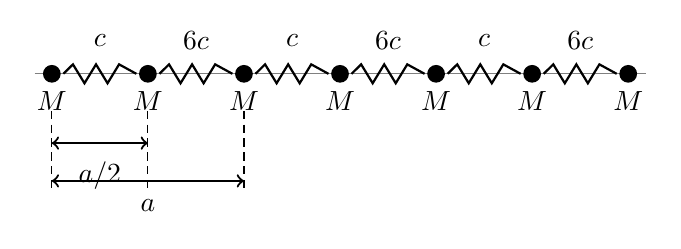
\begin{tikzpicture}[x=1.22cm,y=1cm]
  \draw[gray] (-0.18,0)--(6.18,0);
  \foreach \x in {0,...,6}{\fill (\x,0) circle (3.2pt); \node at (\x,-0.34) {$M$};}
  \foreach \x in {0,...,5}{
    \pgfmathsetmacro{\xA}{\x+0.12}\pgfmathsetmacro{\xB}{\x+0.88}
    \draw[thick] (\xA,0)--({\x+0.22},0.12)--({\x+0.34},-0.12)--({\x+0.46},0.12)--({\x+0.58},-0.12)--({\x+0.70},0.12)--(\xB,0);
    \ifodd\x \node[fill=white,inner sep=1.5pt] at ({\x+0.50},0.42) {$6c$};
    \else \node[fill=white,inner sep=1.5pt] at ({\x+0.50},0.42) {$c$};\fi
  }
  \foreach \x in {0,1,2}{\draw[densely dashed] (\x,-0.47)--(\x,-1.48);}
  \draw[<->,thick] (0,-0.88)--(1,-0.88) node[midway,below=3pt] {$a/2$};
  \draw[<->,thick] (0,-1.36)--(2,-1.36) node[midway,below=3pt] {$a$};
\end{tikzpicture}
\end{center}
\begin{enumerate}
  \item 求 $k=0$ 和 $k=\pi/a$ 处各支格波的频率。（6 分）
  \item 在第一布里渊区内定性画出色散关系。（4 分）
\end{enumerate}


\begin{solution}
以每个周期 $a$ 中的两个原子位移为 $u_n,v_n$，令 $c$ 为胞内弹簧、$6c$ 为相邻胞之间弹簧。运动方程为
\[
\begin{aligned}
 M\ddot u_n&=-c(u_n-v_n)-6c(u_n-v_{n-1}),\\
 M\ddot v_n&=-c(v_n-u_n)-6c(v_n-u_{n+1}).
\end{aligned}
\]
代入
$u_n=U\ee^{\ii(kna-\omega t)}$、
$v_n=V\ee^{\ii(kna-\omega t)}$，得到
\[
 \begin{vmatrix}
 7c-M\omega^2&-(c+6c\ee^{-\ii ka})\\
 -(c+6c\ee^{\ii ka})&7c-M\omega^2
 \end{vmatrix}=0.
\]
因此
\[
 \boxed{M\omega_\pm^2=7c\pm c\sqrt{37+12\cos ka}.}
\]
其中负号为声学支，正号为光学支。

在 $k=0$，根号为 7：
\[
 \boxed{\omega_-(0)=0,\qquad \omega_+(0)=\sqrt{\frac{14c}{M}}.}
\]
在区边界 $k=\pi/a$，根号为 5：
\[
 \boxed{\omega_-(\pi/a)=\sqrt{\frac{2c}{M}},\qquad
 \omega_+(\pi/a)=\sqrt{\frac{12c}{M}}.}
\]
色散关于 $k=0$ 偶对称；声学支从 0 单调升至
$\sqrt{2c/M}$，光学支从 $\sqrt{14c/M}$ 单调降至
$\sqrt{12c/M}$，两支之间存在频率隙。
\begin{center}
\begin{tikzpicture}[x=1.02cm,y=0.78cm]
  \draw[->] (-3.45,0)--(3.55,0) node[right] {$k$};
  \draw[->] (0,0)--(0,4.30) node[above] {$\omega$};
  \draw[domain=-3.1416:3.1416,samples=180,very thick] plot (\x,{sqrt(7-sqrt(37+12*cos(\x r)))});
  \draw[domain=-3.1416:3.1416,samples=180,very thick] plot (\x,{sqrt(7+sqrt(37+12*cos(\x r)))});
  \draw[densely dashed] (-3.1416,0)--(-3.1416,3.60);
  \draw[densely dashed] (3.1416,0)--(3.1416,3.60);
  \node[below=3pt] at (-3.1416,0) {$-\pi/a$}; \node[below=3pt] at (0,0) {$0$}; \node[below=3pt] at (3.1416,0) {$\pi/a$};
  \fill (0,0) circle (2pt); \fill (0,{sqrt(14)}) circle (2pt);
  \fill (-3.1416,{sqrt(2)}) circle (2pt); \fill (3.1416,{sqrt(2)}) circle (2pt);
  \fill (-3.1416,{sqrt(12)}) circle (2pt); \fill (3.1416,{sqrt(12)}) circle (2pt);
  \node[anchor=south east] at (-0.28,3.92) {$\sqrt{14c/M}$};
  \draw[->] (-0.24,3.83)--(-0.04,3.76);
  \node[anchor=west] at (2.00,4.00) {光学支};
  \draw[->] (2.18,3.86)--(2.48,3.56);
  \node[anchor=west] at (2.00,0.68) {声学支};
  \draw[->] (2.18,0.82)--(2.48,1.18);
\end{tikzpicture}
\end{center}
\end{solution}
\end{question}

\begin{question}[10 分]
在 Debye 模型近似下，讨论由 $N$ 个原子组成的二维正方晶格的热容。
\begin{enumerate}
  \item 推导晶格热容的表达式。（6 分）
  \item 求高温极限和低温极限下的热容。（4 分）
\end{enumerate}
计算中可取
\[
  \theta_{\mathrm D}=\frac{\hbar\omega_{\mathrm D}}{k_{\mathrm B}},\qquad
  x=\frac{\hbar\omega}{k_{\mathrm B}T},\qquad
  \int_0^\infty\frac{x^3\ee^x}{(\ee^x-1)^2}\,\dd x=\alpha.
\]


\begin{solution}
二维晶体有两条声学支。Debye 近似取线性色散 $\omega=vq$，二维圆形 $q$ 空间内的模式数正比于 $q^2$，故态密度为
\[
 g(\omega)=C\omega.
\]
由总模数 $2N$ 归一化：
\[
 \int_0^{\omega_D}C\omega\,\dd\omega=2N
 \quad\Longrightarrow\quad
 \boxed{g(\omega)=\frac{4N}{\omega_D^2}\omega.}
\]
忽略零点能，内能为
\[
 U=\int_0^{\omega_D}
 \frac{\hbar\omega}{\ee^{\hbar\omega/(k_BT)}-1}g(\omega)\,\dd\omega.
\]
令 $x=\hbar\omega/(k_BT)$、$x_D=\theta_D/T$，则直接对 Bose 占据数求导可得
\[
 \boxed{C_V=4Nk_B\left(\frac{T}{\theta_D}\right)^2
 \int_0^{\theta_D/T}
 \frac{x^3\ee^x}{(\ee^x-1)^2}\,\dd x.}
\]

高温 $T\gg\theta_D$ 时每个谐振子自由度贡献 $k_B$，或在积分中用
$\ee^x/(\ee^x-1)^2\simeq x^{-2}$，得到
\[
 \boxed{C_V\longrightarrow2Nk_B.}
\]
低温 $T\ll\theta_D$ 时上限可延至无穷，题给积分为 $\alpha$，故
\[
 \boxed{C_V\simeq4\alpha Nk_B
 \left(\frac{T}{\theta_D}\right)^2.}
\]
这就是二维 Debye 模型的 $T^2$ 定律。
\end{solution}
\end{question}
